\documentclass[tikz,border=6pt]{standalone}
\usepackage{pgfplots}
\pgfplotsset{compat=1.18}

\begin{document}
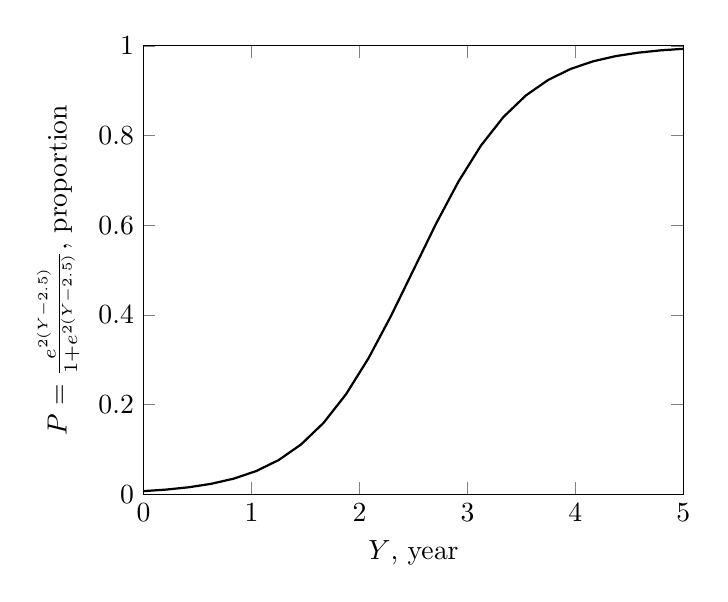
\begin{tikzpicture}
\begin{axis}[
    xlabel={$Y$, year},
    ylabel={$P=\frac{e^{ 2(Y-2.5)}}{1+e^{ 2(Y-2.5)}}$, proportion},
    xmin=0, xmax=5,
    ymin=0, ymax=1,
]
    % Gráfica de y = e^x
    \addplot[domain=0:5, thick] {exp(2*(x-2.5))/(1+exp(2*(x-2.5)))};
\end{axis}
\end{tikzpicture}
\end{document}